\chapter{Results}
\begin{toDo}
	\section{Architecture}
	Come accennato nei capitoli precedenti, il sistema di analisi delle immagini richiede di confrontare l'opera sconosciuta con quelle note.

	\noindent L'immagine viene preprocessata rimuovendo elementi inquinanti che non riguardano la grafia, lasciando essenzialmente un'immagine in scala di grigi con la grafia dell'autore in tonalità scura e lo sfondo bianco. Inoltre, il tratto dell'autore potrebbe necessitare di uno spessore specifico rispetto ai caratteri impressi e la risoluzione (espressa in \gls{dpi}) deve essere conforme al dataset.

	\noindent L'immagine così preprocessata sarà quindi sintetizzata: un programma ne estrae tutte le tessere con una dimensione specifica conforme al dataset. In seguito, l'immagine sarà confrontata con ogni immagine del dataset (o con le più rappresentative per ogni autore).

	\noindent In questo capitolo si effettueranno analisi di ogni passaggio illustrato in questa tesi al fine di vedere come ogni singola componente agisce sulle immagini esaminate. Non solo, si mostreranno anche le analisi effettuate per stabilire specifiche decisioni e parametri usati durante la fase di progettazione.

	\bigskip\noindent La costruzione del dataset avviene con un procedimento lievemente diverso. Ogni immagine di cui l'autore è noto viene confrontata completamente con tutte le altre già note. Essendo l'indice di dissimilarità simmetrico, sarà sufficiente esaminare la metà di tutti i confronti possibili. Se si è in possesso di $n$ immagini, pensiamo di voler riempire una tabella quadrata $n\times n$ con valori reali. Assumendo dissimilarità $0$ tra immagini con se stesse, si può concludere che in totale saranno richiesti $\frac{n^2-n}{2}$ confronti.

	\noindent Per questa ragione, l'algoritmo per ogni riga esaminerà la metà dei possibili confronti come mostrato in \cref{fig:distance_computation}. In particolare, se $n$ è dispari, per ogni riga si faranno $\frac{n-1}{2}$ confronti (e altrettanti saranno memorizzati per via della simmetria), mentre se $n$ è pari, allora $\frac{n}{2}$ confronti saranno effettuati se la riga $i$ è pari (la prima riga ha indice $0$) e $\frac{n}{2}-1$ se la riga $i$ è dispari. Questa procedura permette una analisi più uniforme ed efficiente per numerosi dati, specie se accompagnata da shuffle per riga e per colonna.

	\begin{figure}[h]
		\centering
		\includegraphics[width=0.7\linewidth]{Figures/analysis_sort.png}
		\caption[Visit all couples]{The algorithm for each row computes half of all components. In the image, the algorithm follows the order of the numbers and alternately takes the cells such that the lower diagonal is not directly computed and the upper diagonal is directly computed. For example, in the $3^\text{-th}$ row, the algorithm computes directly the first column (number $5$ in cyan) and the next-to-last column (number $6$ in cyan), while the second column is already computed (number $3$ in green square) and the last column is not yet computed.}
		\label{fig:distance_computation}
	\end{figure}

	\subsection{Challenges}
	L'implementazione del codice ha richiesto notevoli sforzi poiché gran parte dei framework richiesti non erano esistenti, inoltre le limitazioni della potenza di calcolo e il tempo a disposizione hanno rappresentato un forte vincolo. Questo ha richiesto la stesura di codice altamente prestante e sofisticato per ottimizzare l'efficienza computazionale.

	\noindent In generale, il progetto ha richiesto largo uso di \gls{Python} e \gls{CUDA}. Durante la sua realizzazione si sono utilizzati software specifici per debugging, logging e testing, utili per monitorare il corretto funzionamento del software. Sono stati impiegati strumenti di documentazione automatica e gestione delle versioni del codice. Inoltre, è stato adottato un robusto sistema di gestione degli errori e delle sessioni di calcolo, con meccanismi di backup (detti "checkpoint") per scongiurare la perdita di dati preziosi. Il software utilizza anche file temporanei per aumentare la capacità di memorizzazione oltre i limiti della memoria principale.

	\noindent Per queste ragioni, il codice (composto da un totale di $3480$ righe) è difficilmente riportabile per intero in questo testo ed è consultabile nella repository \gls{github}:\\ \url{https://github.com/StefanoMagriniAlunno/MMATH_thesis}.

	\bigskip\noindent La macchina che ha prodotto i risultati illustrati in questo capitolo ha le seguenti specifiche tecniche:
	\texttt{\begin{itemize}
		\item \textbf{processor}: 11th Gen Intel(R) Core(TM) i7-11370H @ 3.30GHz
		\begin{itemize}
			\item[-] Cores: 4
			\item[-] Thread(s) per core: 2
			\item[-] CPU max MHz: 4800
			\item[-] Caches:
			\begin{itemize}
				\item[*] L1d 192KiB (4 instances)
				\item[*] L1i 128KiB (4 instances)
				\item[*] L2 5MiB (4 instances)
				\item[*] L3 12MiB (1 instances)
			\end{itemize}
		\end{itemize}
		\item \textbf{memory}: 16 GiB
		\begin{itemize}
			\item[-] SODIMM DDR4 Synchronous 3200 MHz (0,3 ns)
			\item[-] SODIMM DDR4 Synchronous 3200 MHz (0,3 ns)
		\end{itemize}
		\item \textbf{memory}: 16 GiB
		\begin{itemize}
			\item[-] SODIMM DDR4 Synchronous 3200 MHz (0,3 ns)
			\item[-] SODIMM DDR4 Synchronous 3200 MHz (0,3 ns)
		\end{itemize}
		\item \textbf{graphic processor unit}: NVIDIA GeForce GTX 1650
		\begin{itemize}
			\item[-] Cores: 896
			\item[-] stream multiprocessor: 14
			\item[-] VRAM: GDDR5 4096 MiB
			\item[-] CUDA capability: 7.5
		\end{itemize}
	\end{itemize}}
	\noindent Saranno visionate anche le prestazioni per sottolineare come l'uso di processori grafici possa essere estremamente utile per questo tipo di fini.

	\bigskip\noindent Il codice fa uso di wrapping, ossia di programmi in grado di far scorrere il flusso di uno script di \gls{Python} in un codice precompilato di \gls{cxx}.In questo modo si è realizzato con codice \gls{Python} uno script di avvio per le sessioni di calcolo che prepara file e report utili, recupera specifiche hardware e configurazioni del calcolo da eseguire. Laddove è richiesto un'intensivo calcolo lo script \gls{Python} chiamerà una libreria precompilata scritta in \gls{cxx}. In questo modo il codice \gls{cxx} potrà essere più essenziale e quindi leggibile.

	\noindent Per fare un esempio di avvio di una comparazione tra opere, lo script principale di \gls{Python} si occupa di preparare il sistema operativo, convalidare i parametri usati ed eventuali checkpoint. Quindi, fornisce tutti gli input richiesti al wrapper (scritto in \gls{cxx}) il quale convalida eventuali errori di sintassi e traduce i tipi di valori di \gls{Python} in tipi comprensibili al \gls{cxx}. Di seguito, questi valori vengono passati ad uno starter che prepara un logger e legge eventuali file inizializzando di fatto la memoria principale. Il programma scritto in \gls{cxx} chiama il programma scritto in \gls{CUDA} il quale si occupa di leggere i dettagli tecnici della \gls{gpu} (usando apposite librerie) per configurare un piano di calcolo che massimizza le prestazioni e che sia robusto. Infine, verranno comunicate le istruzioni alla \gls{gpu} come kernel (codice esplicito che compilerà la \gls{gpu} stessa in runtime). Poiché la memoria della \gls{gpu} è limitata, è importante far attenzione che i dati siano passati parzialmente e usare la memoria principale come appoggio.

	\noindent I dati ottenuti dalla \gls{gpu} vengono passati alla funzione chiamante in \gls{cxx} la quale li memorizza in modo opportuno e restituisce il controllo allo script di \gls{Python} chiamante. In caso di errori tutto viene documentato e riportato al chiamante per gestirli in modo opportuno.

	\noindent Questo tipo di strategie per realizzare codice prestante sono tipiche nelle librerie di calcolo scientifico che spesso mostrano una funzione principale chiamante e funzioni compilate nascoste, un esempio è CuPy, una libreria \gls{Python} la quale installazione prevede anche la compilazione.

    \section{Pre processing}
    Il pre processing è una fase importante del confronto tra opere ignote con il dataset. In particolare si preoccupa di far rispettare delle specifiche qualitative dell'immagine per lo più soggettive, non è quindi detto che si faccia uso dello stesso algoritmo per ogni immagine. Il fine ultimo è eliminare dati evidentemente inquinanti per far rispettare un certo standard e presentare l'immagine al software nel giusto modo. Essenzialmente si avvicina il dato reale al dato ideale ammissibile teoricamente dal software.

    \noindent Come già illustrato in \cref{alg:CleaningFFT}, il preprocessing adottato per i dati raccolti fa uso principalmente di una compressione con \gls{fft}. In questa sezione saranno illustrati i risultati passo passo seguendo l'algoritmo.

    \paragraph{FFT}
    Il primo step dell'algoritmo di preprocessing è applicare \gls{fft} all'immagine normalizzata, quindi con pixel grigi aventi valori di media $0$ e varianza $1$. Come osservato, attraverso immagini sintetiche, i quadretti nello sfondo delle pagine di appunti sono pattern ricorrenti che tipicamente non sono propri della scrittura di un testo. Questa ricorrenza è meglio visibile attraverso l'uso di trasformate di Fourier.

   	\noindent In \cref{fig:fft_application} è visibile il pattern dei quadretti come frequenze alte separatamente su $x$ e su $y$ di significiativa intensità.

    \begin{figure}[h]
    	\centering
    	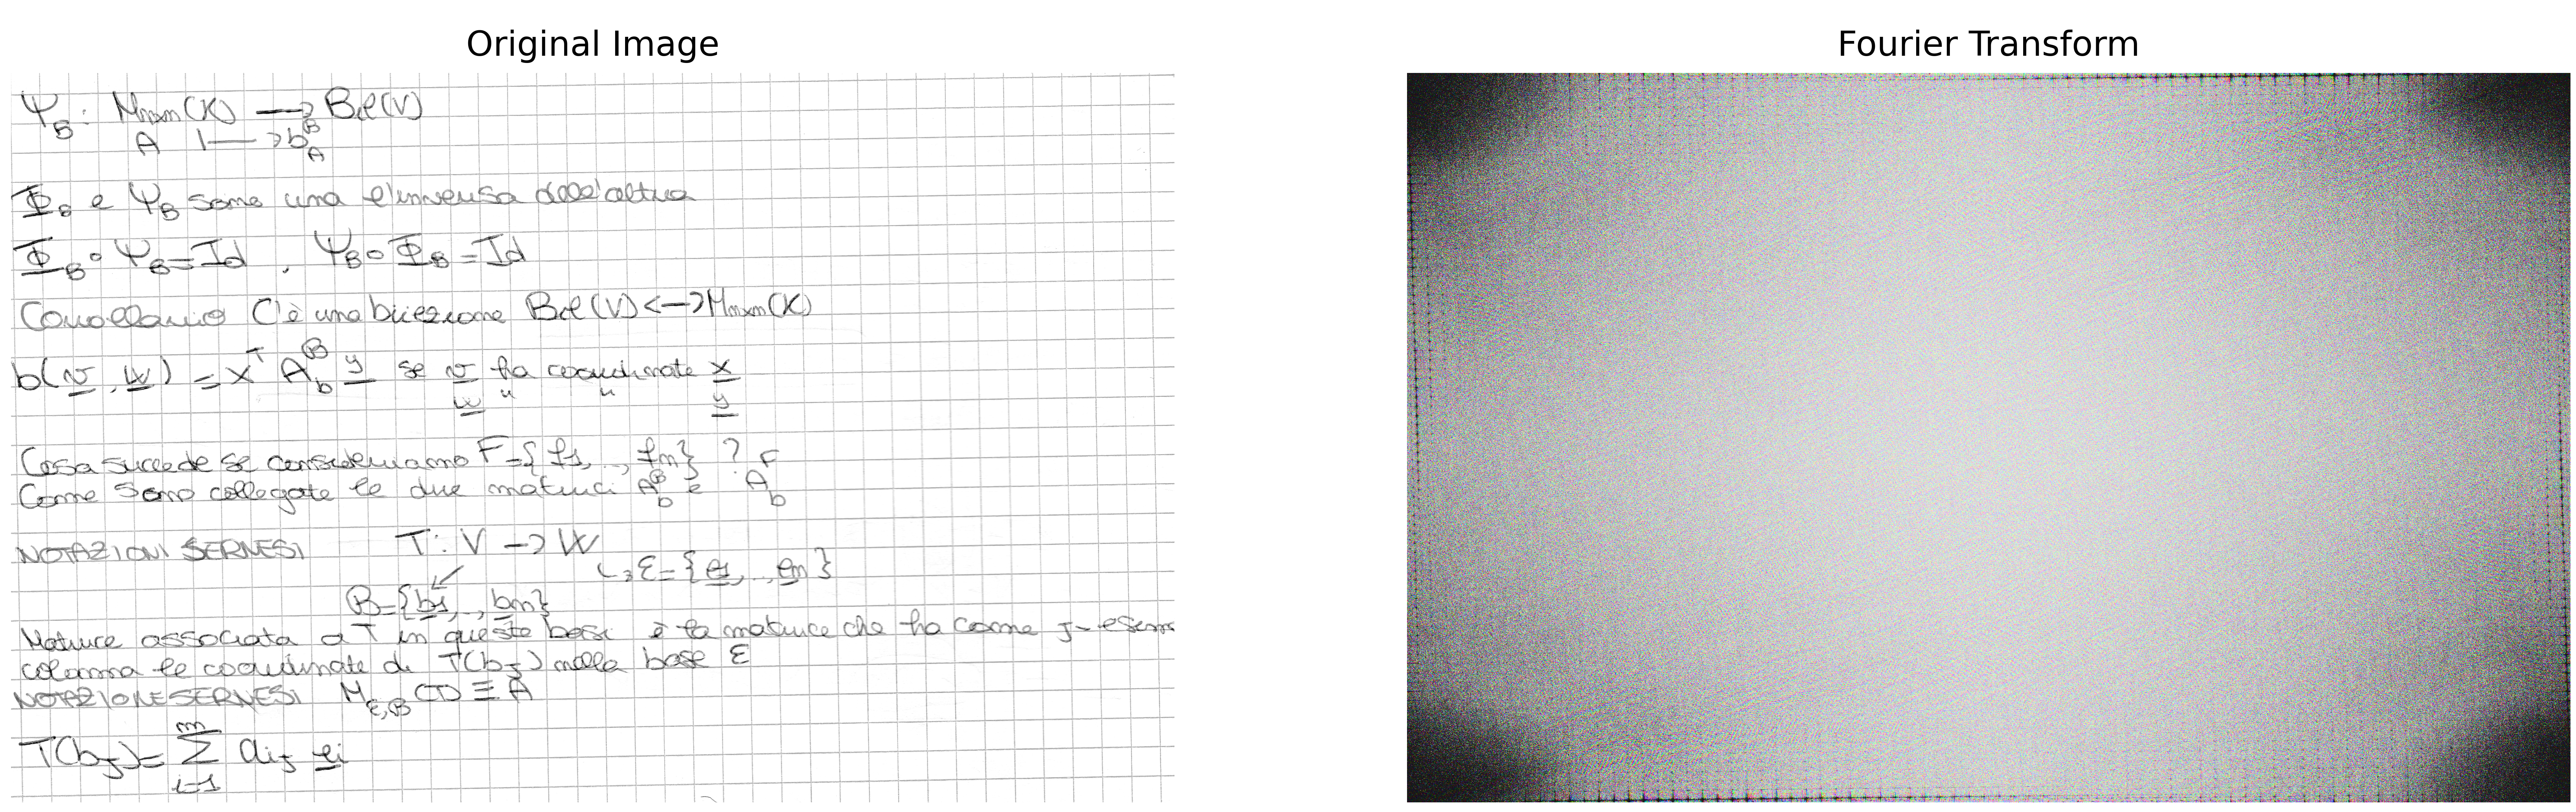
\includegraphics[width=1.0\linewidth]{Figures/fft_application.png}
    	\caption[fft application]{We can observe significant frequencies along the edge of the second image. The template of the sheet is captured from \gls{fft}, the frequencies along the edges are high for an ax and low for the other ax.}
    	\label{fig:fft_application}
    \end{figure}

	\noindent Il programma rimuove il $p$-percentile delle frequenze con più alta intensità. Dopodiché ricostruisce l'immagine originale usando le frequenze rimaste, cui intensità non è stata annullata. In \cref{fig:fft_percentile} si vedono varie ricostruzioni usando differenti percentili e una normalizzazione tra $0,1$ dei grigi ottenuti. Osserviamo come $p=0.1\%$ è una scelta appropriata da cui cominciare le analisi.

	\begin{figure}[h]
		\centering
		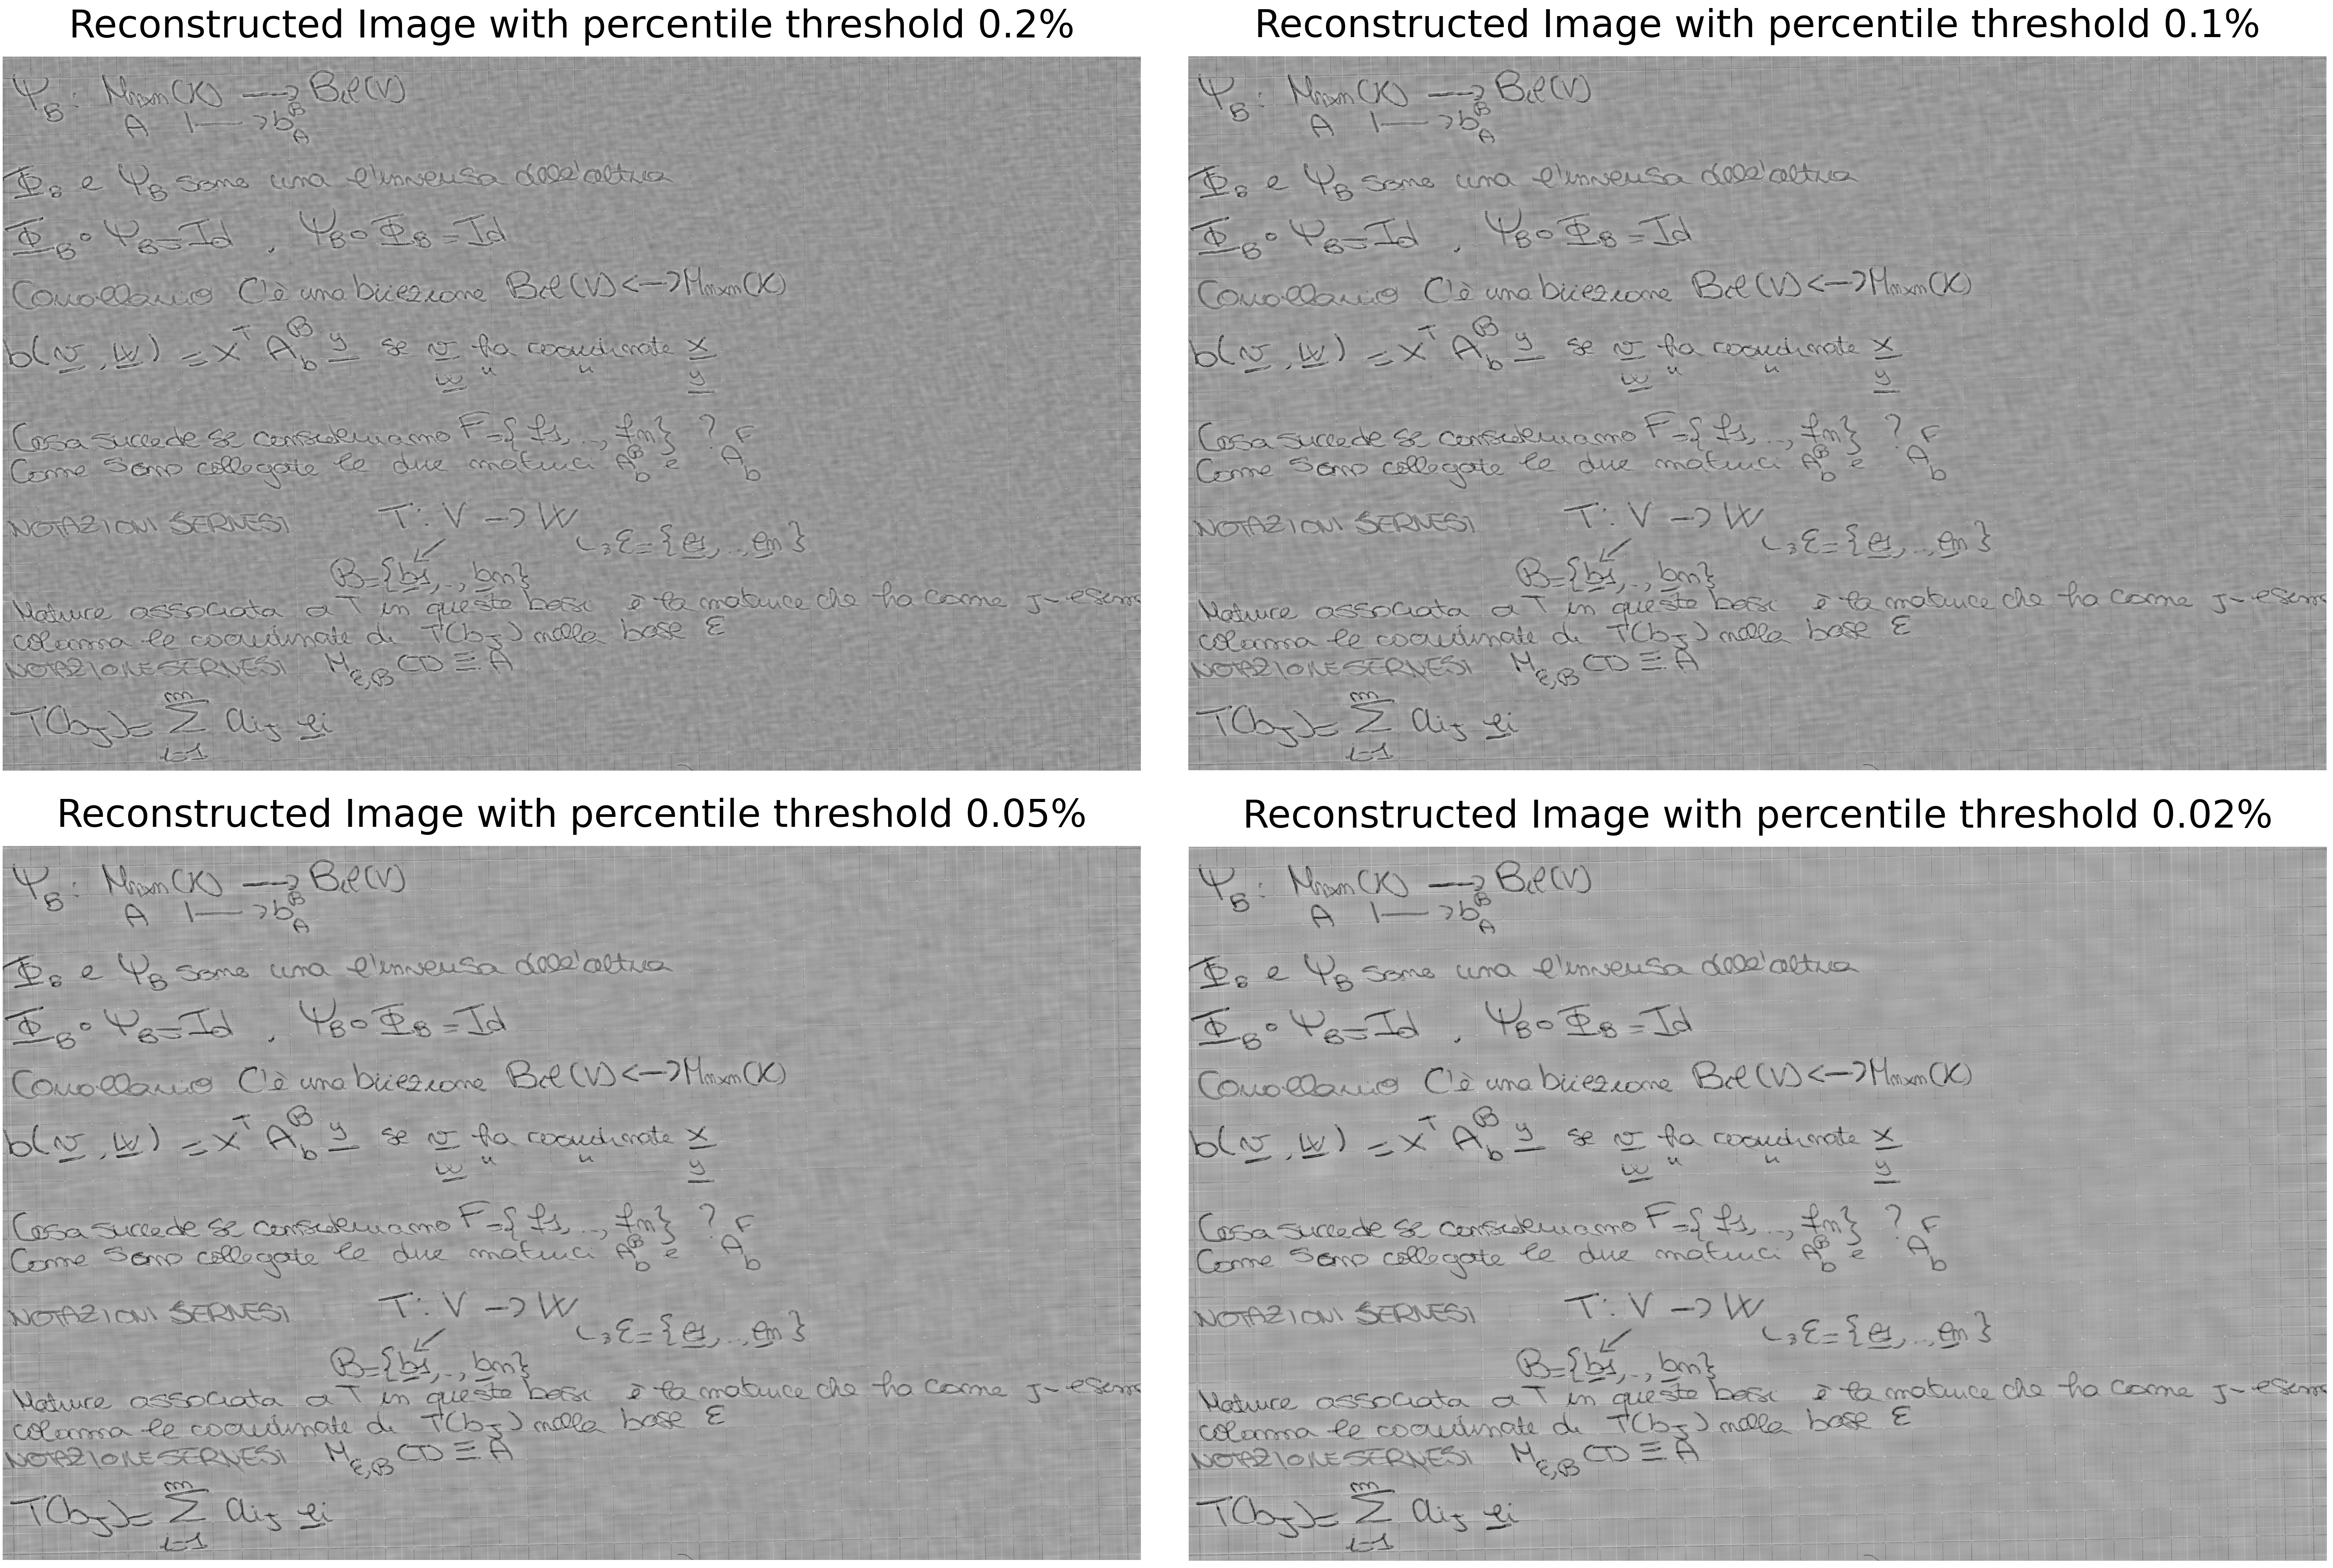
\includegraphics[width=0.8\linewidth]{Figures/fft_percentile.png}
		\caption[comparing different percentiles in fft]{Si può osservare che un percentile tra $0.1\%$ e $0.05\%$ è un buon compromesso, i quadretti sembrano sparire e la scrittura rimane intaccata.}
		\label{fig:fft_percentile}
	\end{figure}

	\noindent Si può osservare che la normalizzazione effettuata per visualizzare queste immagini nasconde il fatto che i pixel sono in realtà tutti visibilmente uguali tra loro. L'idea quindi è individuare quanti pixel erano parte certamente dello sfondo bianco della pagina e quanti invece delle grafie. Analizzando le immagini si è osservato che i pixel con valore di grigio inferiore a $0.2$ sono certamente parte delle grafie, invece se il valore è superiore a $0.8$ sono certamente parte dello sfondo bianco della pagina. Quindi l'algoritmo recupera quanti pixel sono certamente delle grafie e quanti lo sono per la scrittura. In figura \cref{fig:fft_diagrams} un'illustrazione di questa analisi.

	\begin{figure}[h]
		\centering
		\includegraphics[width=0.8\linewidth]{Figures/fft_diagrams.png}
		\caption[different density after fft compression]{Nell'immagine originale si osserva che la densità dei grigi presentava, per ovvie ragioni, molti pixel bianchi. Mentre nell'immagine ricostruita sono per lo più grigi medi. Per mantenere una distribuzione quanto meno simile a quella di partenza bisogna separare di più i colori tra loro. Per questa ragione si contano quanti pixel avevano un livello grigio superiore ad un certo threshold che ne certifichi l'appartenenza allo sfondo, così anche per la quantità di pixel sufficientemente scuri da considerarsi parte delle grafie.}
		\label{fig:fft_diagrams}
	\end{figure}

	\noindent Noti i due estremi nell'immagine ricostruita, si esegue una trasformazione lineare dei livelli di pixel che fa sì che gli estremi abbiano livelli rispettivamente $0$, $1$:
	\[
		\texttt{gray}_\texttt{new} = \frac{\texttt{gray}_\texttt{old} - \texttt{h}_\texttt{low}}{\texttt{h}_\texttt{up} - \texttt{h}_\texttt{low}}
	\]
	dove $\texttt{h}_\texttt{low}$ e $\texttt{h}_\texttt{up}$ indicano i threshold nell'immagine ricostruita. Di conseguenza i pixel con un livello inferiore a $0$ o superiore a $1$ saranno resi automaticamente $0$, $1$, rispettivamente, usando la trasformazione \texttt{clamp}.

	\noindent In \cref{fig:fft_results} si mostrano i risultati di questo processo per percentili $0.1\%$ e $0.05\%$ su $2$ campioni. Come si osserva, il risultato non è molto differente ad occhio nudo. Per preservare meglio le grafie, a costo di lasciare più segni di quadretti, si è deciso di usare $p=0.05\%$. L'idea è sperare che questo rumore sia in qualche modo catturato dal clustering fuzzy.

	\begin{figure}[h]
		\centering
		\includegraphics[width=1.0\linewidth]{Figures/fft_results.png}
		\caption[results of "fft cleaner"]{In figura sono mostrate due immagini preprocessate usando differenti percentili. La prima colonna fa uso di $p=0.05\%$, la seconda di $p=0.1\%$, ogni riga fa riferimento ad un'opera del dataset.}
		\label{fig:fft_results}
	\end{figure}

    \section{Synthesis}
    Una volta che le immagini sono state preprocessate e quindi rese conformi al dataset secondo parametri "umani", si procede con la sintesi che di fatto rende le opere conformi da un punto di vista oggettivo. In particolare le opere saranno ridefinite come un elenco (ordinato o meno) delle loro tessere che saranno quadrate e aventi la stessa forma.

    \noindent Come già accennato, lo script \gls{Python} si occupa di preparare il sistema operativo e ricavare velocemente input e parametri hardware per i programmi precompilati a più basso livello. In questo caso lo script \texttt{synthesis.py} in poche linee di codice crea le cartelle utili nelle quali un programma \gls{cxx} può memorizzare le sintesi ottenute con il seguente loop:

\begin{lstlisting}[style=code, language=C, rulecolor=\color{blue}]
/** @brief In this code we use OpenMP API to realize an array with all tiles.
 *
 *  @param[in] byte_board : the array with all pixels
 *  @param[out] cells : the array with all tiles of the image
 *  @param n_threads : the number of used threads in the first loop
 *  @param height : the height of the image
 *  @param width : the width of the image
 *  @param n_tiles : the size of tiles
 *
 *  @details This code uses a bijective map from tiles and "short"image, i.e. an image with shape width_short, height_short. Each tiles will be assigned to its first pixel (up/sx).
 *           "omp parallel for" is a directive of OpenMP that executes a for cycle using more indipendent threads. In this case the schedule is "static" i.e. each thread knows in advance all its loops.
 */
unsigned width_short = width - n_tiles + 1,
         height_short = height - n_tiles + 1;
#pragma omp parallel for schedule(static) num_threads(n_threads)
for (unsigned row = 0; row < height_short; ++row)
for (unsigned col = 0; col < width_short; ++col)
    for (unsigned i = 0; i < n_tiles; ++i)
    for (unsigned j = 0; j < n_tiles; ++j) {
        long unsigned index_out = ((row * width_short + col) * n_tiles + i) * n_tiles + j; // [row-i, col-j, i,j]
        long unsigned index_in = (row + i) * width + col + j;
        cells[index_out] = byte_board[index_in];
    }\end{lstlisting}

    \paragraph{Details}
    Usare più \gls{thread} per compiere un ciclo aiuta ad aumentare le prestazioni del ciclo di un fattore moltiplicativo. In questo caso non si temono nemmeno problemi di concorrenza, ossia più \gls{thread} che scrivono sulla medesima cella di memoria. In questo caso il tempo di esecuzione nominale di un loop non dipende dalla scelta della riga, per questa ragione una schedule statica riduce di molto anche i tempi stessi per gestire il gruppo di thread generati.

    \noindent La tecnica del multi-threading si usa per ottimizzare i tempi di esecuzione di piccoli passaggi parallellizzabili. E' quindi inusuale vedere applicati questo tipo di algoritmi a

    Mostrare una piccola analisi delle sintesi ottenute e della velocità del programma, magari con dettagli implementativi
    \section{Comparison}
   		Mostrare dettagli del clustering a livello esecutivo, come velocità del programma e confronto con l'esecuzione su CPU
    	\subsection{Results}
    		Mostrare dettagli in esecuzione dei vari valori ottenuti dall'algoritmo di comparazione. Quindi concludere con una panoramica dei risultati ottenuti.
\end{toDo}


%\begin{figure}
%	\centering
%	\includegraphics[width=\linewidth]{Figures/first_reconstruct.png}
%	\caption{Come si osserva i grigi si sono molto avvicinati tra loro dopo \gls{fft}, ma è possibile ribilanciare i colori confrontandoli con l'immagine originale.}
%	\label{fig:first_reconstruct}
%\end{figure}
